\section{Gerenciamento}

\subsection{SCRUM}

Scrum é uma metodologia ágil para gestão e planejamento de projetos de software. \cite{scrum}.

De acordo com \cite{scrum}, os projetos são divididos em ciclos ou iterações (tipicamente mensais) chamados de
\textit{Sprints}.  As \textit{Sprints} representam um \textit{Time Box}, ou seja, é uma janela de tempo para a execução de um trabalho, dentro do qual um conjunto de atividades devem ser executados.

As funcionalidades a serem implementadas no projeto são mantidas em uma lista chamada \textit{Product Backlog}. Essa lista contém todas as funcionalidades desejadas para um produto sendo elas tarefas técnicas ou atividades diretamente relacionadas às funcionalidades solicitadas, por exemplo, documentação. No início de cada \textit{Sprint}, faz-se um \textit{Sprint Planning}, ou seja, uma reunião de planejamento na qual o \textit{Product Owner} prioriza os itens do \textit{Product Backlog} e equipe seleciona as atividades que ela irá implementar durante a \textit{Sprint} que se inicia. As tarefas alocadas em uma \textit{Sprint} são transferidas do \textit{Product Backlog} para o \textit{Sprint Backlog}, que é uma lista de tarefas que o \textit{Scrum Team}, equipe de 6 a 10 pessoas responsável pelo desenvolvimento do software e pelos testes, se compromete a fazer em uma \textit{Sprint}. \cite{scrum}

O \textit{Scrum Master} procura assegurar que a equipe respeite e siga os valores e as práticas do Scrum. Ele também protege a equipe assegurando que ela não se comprometa excessivamente com àquilo que é capaz de realizar durante uma \textit{Sprint}. Esse papel é tipicamente exercido por um gerente de projeto ou um líder técnico, mas em princípio pode ser qualquer membro da equipe.

A cada dia de uma \textit{Sprint}, a equipe faz uma breve reunião, normalmente 15 minutos, chamada \textit{Daily Scrum}, nessa reunião todos os membros da equipe deve participar, é uma excelente forma para uma equipe disseminar informações sobre o estado do projeto. O objetivo é disseminar conhecimento sobre o que foi feito no dia anterior, identificar impedimentos e priorizar o trabalho do dia que se inicia. Na reunião é feito três perguntas: O que você fez ontem? O que você fará hoje? E há algum impedimento no seu caminho? Com isso a equipe inteira ganha compreensão sobre que trabalho foi feito e que trabalho ainda precisa ser feito. É uma reunião no qual membros da equipe assumem compromissos perante os demais e o \textit{Scrum Master} trata os impedimentos coletados o mais rápido possível. \cite{scrum}

Ao final de uma \textit{Sprint}, o \textit{Scrum Team} apresenta as funcionalidades implementadas em uma \textit{Sprint
Review Meeting}.  Participantes do \textit{Sprint Review} tipicamente incluem o \textit{Product Owner}, o \textit{Scrum
Team}, o \textit{Scrum Master}, gerência, clientes entre outros \textit{stakeholders}. Finalmente, faz-se uma \textit{Sprint Retrospective} para coletar pontos positivos, negativos e melhorias para as próximas iterações da equipe. Com isso a equipe parte para o planejamento da próxima \textit{Sprint}. Assim reinicia-se o ciclo. \cite{scrum}

A figura \ref{fig:scrum} ilustra todos estes passos \cite{scrum}.

\begin{figure}[h!]
	\centering
  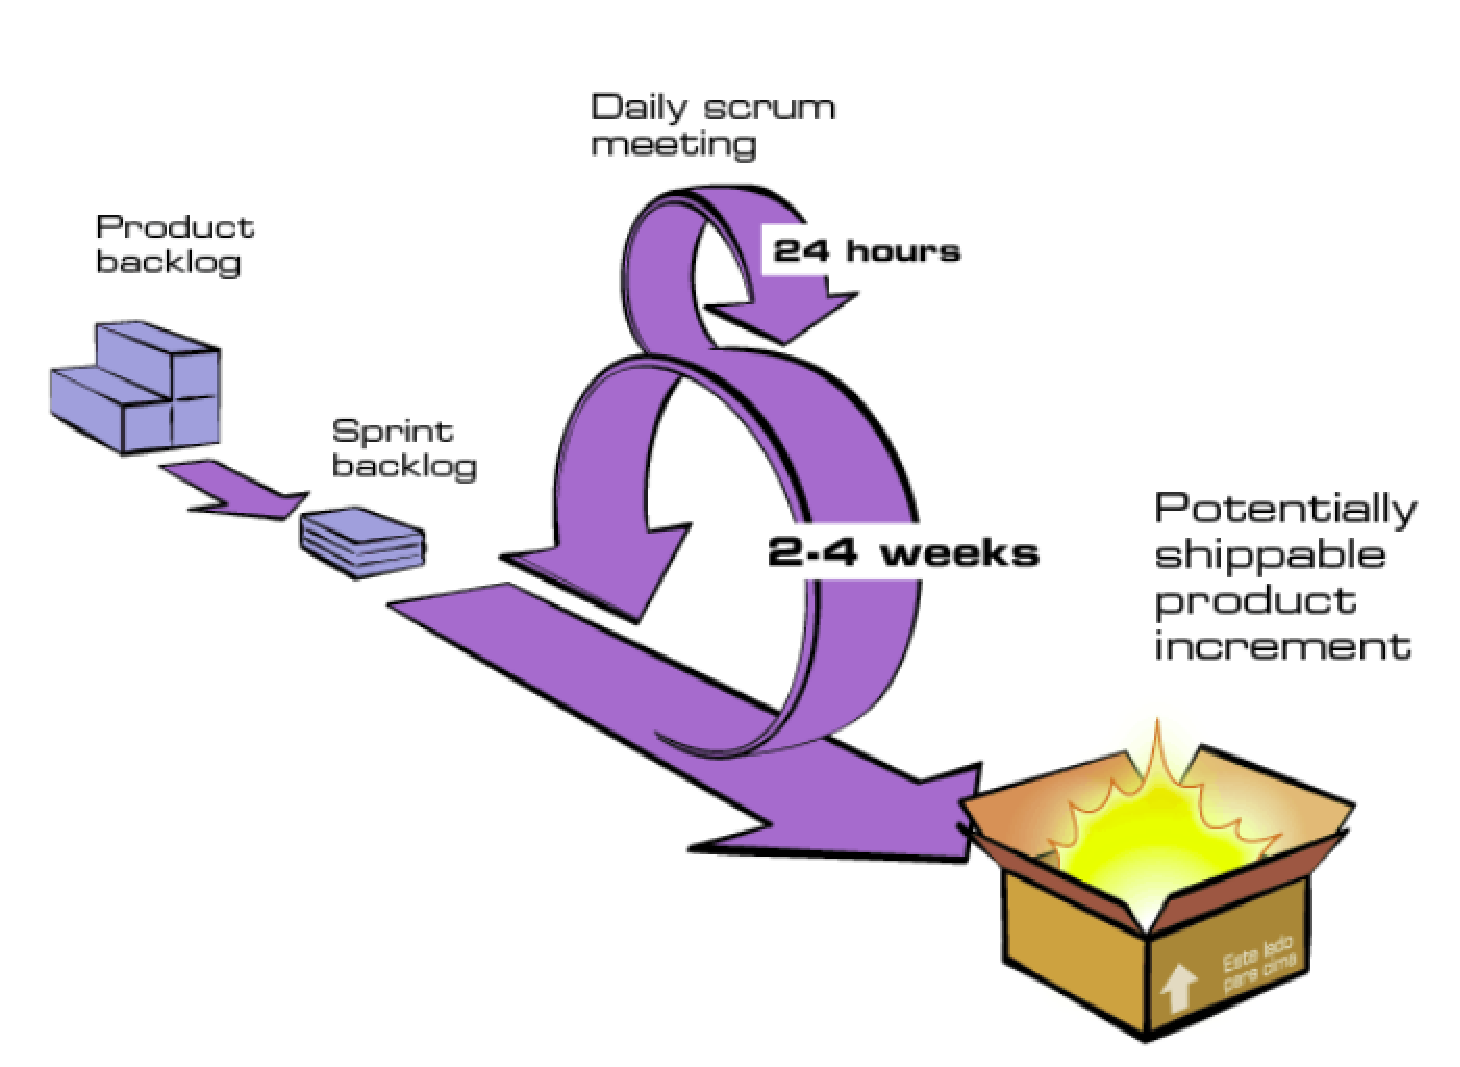
\includegraphics[keepaspectratio=true,scale=0.5]{figuras/scrum.eps}
  \caption{Processo iterativo do SCRUM.}
	\label{fig:scrum}
\end{figure}

\subsection{XP}

\textit{Extreme Programming} ou XP é uma metodologia de desenvolvimento de software que ajuda a criar sistemas de melhor qualidade, que são produzidos em menos tempo e de forma mais econômica que o habitual. Tais objetivos são alcançados através de um pequeno conjunto de valores, princípios e práticas, que diferem da forma tradicional de se desenvolver software. \cite{xp}

\subsubsection{Valores}

\begin{itemize}
  \item \textbf{Comunicação}: A comunicação é essencial para o êxito da metodologia e pode ser realizada de diversas formas, não somente por documentação como nas metodologias tradicionais. A comunicação entre os desenvolvedores instiga a disseminação do conhecimento dentro da equipe, já a comunicação com o cliente garante que o produto entregue atenda à suas expectativas
  \item \textbf{Coragem}: Consiste na coragem durante a implementação de tomar decisões que sejam melhores para a equipe e para o código. Por exemplo, refatorar códigos já implementados para garantir a qualidade do código.
  \item \textbf{Feedback}: O feedback consiste em uma frequente comunicação entre o cliente e a equipe. Dessa forma, a equipe que está desenvolvendo o sistema tem uma visão clara acerca dos requisitos e do que é necessário que seja implementado.
  \item \textbf{Respeito}: Todos os integrantes devem demonstrar respeito uns com os outros.
  \item \textbf{Simplicidade}: Sempre que foi iniciado a implementação de algo, deve ser questionado qual a forma mais fácil de implementar aquele escopo.
\end{itemize}

\subsubsection{Práticas}

\begin{itemize}
  \item \textbf{Testes automatizados}: Teste é o processo de executar um programa ou sistema com a intenção de encontrar defeitos, entre os testes mais conhecidos estão os testes unitários que visa encontrar defeitos em pequenas unidades do software, testes de integração que busca encontrar defeitos na integração entre várias partes do software, testes de aceitação que busca encontrar defeitos nas interfaces do software e testes de regressão que busca encontrar defeitos que foram gerados por novas modificações.
  \item \textbf{Programação pareada}: É uma prática que sugere que o código seja sempre trabalhado em dupla em um mesmo computador, revezando quem está digitando.
  \item \textbf{Refatoração}: É o processo de reorganizar a estrutura interna do software, sem alterar seu comportamento externo, sempre pensando na qualidade do produto.
  \item \textbf{Integração contínua}: A integração contínua é a prática de manter a build sempre estável com novas funcionalidades, ela permite que seja executado testes antes das novas funcionalidades ser integrados no código que irá para o ambiente de produção, ou seja, o ambiente na qual o usuário irá utilizar o software. Isso permite construir confiança e garantir qualidade nas funcionalidades.
  \item \textbf{Entrega contínua}:  A entrega contínua ou deploy contínuo é responsável por automatizar a build do projeto para o ambiente de homologação e produção sem a necessidade de ter alguém intermediando o mesmo. Ele está relacionado diretamente com a integração contínua.
\end{itemize}

\subsection{SAFe}

A engenharia de requisitos é um conjunto de atividades utilizadas para identificar e comunicar a finalidade de um
sistema de software, e o contexto no qual será usado. \cite{leffingwell}

O \textit{Scaled Agile Framework} ou SAFe é uma base de conhecimento on-line, de padrões de sucesso para pessoas que estão construindo softwares e sistemas. Ele descreve as funções, responsabilidades, artefatos e atividades necessárias para implementar o desenvolvimento ágil. O SAFe permite que cada organização o adapte às suas próprias necessidades de negócios, ou seja, suporta soluções de menor escala bem como sistemas complexos. \cite{safe}

Esse tópico irá abordar apenas a rastreabilidade de requisitos do SAFe que será utilizado no projeto. Tendo como
referência, a \textit{The big picture of agile requirements}, por Dean Leffingwell, os temas associados a requisitos, se
dividem, por fases: \cite{safe}

\begin{figure}[h!]
	\centering
  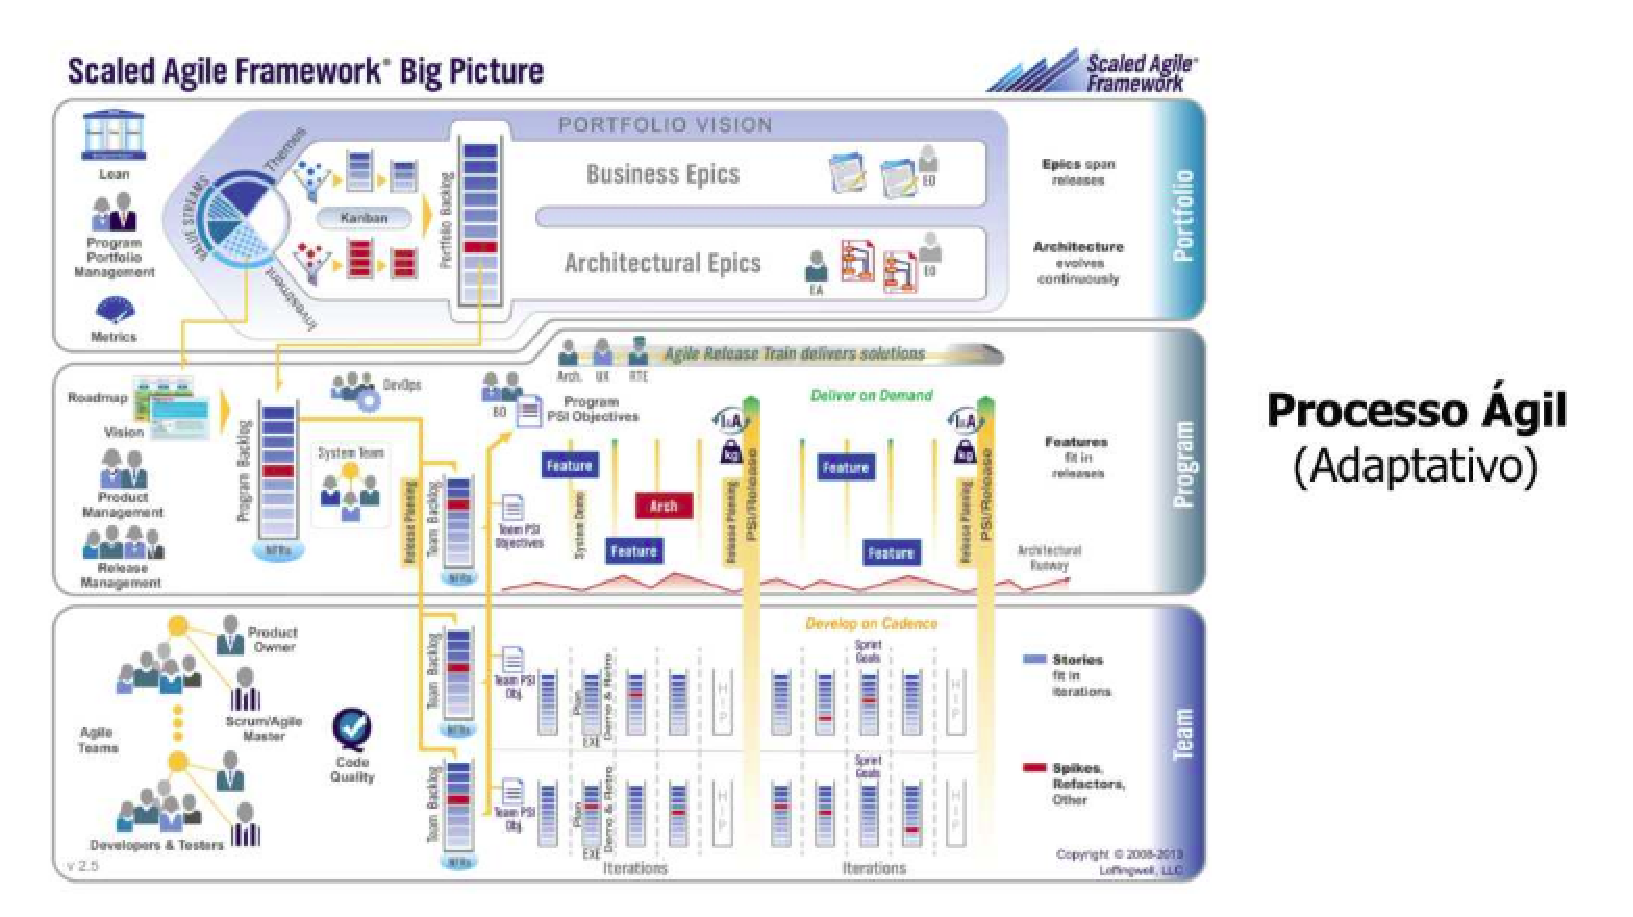
\includegraphics[keepaspectratio=true,scale=0.5]{figuras/safe.eps}
  \caption{Big Picture - SAFe.}
	\label{fig:safe}
\end{figure}

\begin{itemize}
  \item \textbf{Portfólio}: Temas de investimento e Épicos
  \item \textbf{Programa}: Visão, Arquitetura, Features, Requisitos não-funcionais, EAP e Roadmap
  \item \textbf{Time}: Estórias de usuários e tarefas
\end{itemize}

\subsubsection{Portfólio}

Fase responsável por alinhar estratégia de negócio e intenções de investimento, assim que a equipe tem a descrição do valor, isso pode ser quebrado em funcionalidades por meio de épicos, por exemplo, um tema de investimento de um e-commerce tem como épicos, sistema de autenticação/autorização, sistema de vendas, catálogo de produtos, entre outros. É nessa fase que é aplicado a engenharia de requisitos.

\subsubsection{Programa}

Fase responsável pela auto-organização de times ágeis, entrega contínua de valor, criação de Features por meio dos épicos encontrados, realização de toda a documentação relacionada ao \textit{User Experience} ou UX, e definição do documento de arquitetura do software.

\subsubsection{Time}

Fase responsável pelo auto-gerenciamento da equipe ágil, incremento do software totalmente testado, práticas SCRUM e XP, descrição do valor por meio de User Stories e tarefas.

\subsection{Kanban}

O kanban é uma estrutura para implementar o desenvolvimento ágil de software. Os itens de trabalho são apresentados em
quadros do kanban, permitindo que os membros da equipe vejam o estado de cada parte do trabalho a qualquer momento
\cite{dan}.

Os quadros mais comuns do kanban são \textit{TO DO}, \textit{DOING} e \textit{DONE}, que mostra as funcionalidades que deve ser feita, as que estão em progresso e as que já foram completadas respectivamente.
